In this section we will look at a large variety of different simulators, to determine which one best suits our purpose. We will be looking at which operating system and game engine the simulator uses, whether or not it is open source, and the pros and cons of each simulator. We will be particularly looking at the simulators sensing abilities, ability to add additional entities, map customisability, available APIs, and how user-friendly the simulator is. Aspects of the simulator which is not as important as how realistic the simulator physics is, and how visually good looking it is. These are criteria formed by the project specification (Section~\ref{ProjectSpec})
\\~\\
The purpose of this section is to get a good understanding of the different simulators currently in existence. The aim is to find 3-4 simulators that would be worth looking closer at.

%%%%%%%% 4DV-Sim %%%%%%%%%%
\subsection{4DV-Sim}
\textbf{Description:} 4DV-Sim\footnote{Website: \url{https://www.4d-virtualiz.com/en/automotive-simulator}} is a simulator that is designed to emulate the hardware and sensors in autonomous systems. This is a professional product and has a variety of use cases from simulating farming to military equipment \cite{4dv-simulator}.

\textbf{Open Source:} No

\textbf{Operating System:} Linux

\textbf{Game Engine:} Non, but it does use PhysX for the physics engine

\textbf{Pros:} The simulator has a lot of available APIs. The simulator also comes with a configurable GUI to set up the simulation environment how you would like it. Also, as it is professionally made, it looks very good.   

\textbf{Cons:} It is not designed to train machine learning implementations on the simulator, but rather emulate a current hardware setup. Also, as it is not open source, it will not be something that we could modify or expand upon to suit our purposes. 

\textbf{Conclusion:} As 4DV-Sim is not an open-source product it is not something that we can use for this project. It is however interesting to see that simulators like this are needed not just for research purposes, but for customers who want to try out their hardware setup in an emulated environment.


\begin{figure}[H]
    \centering
    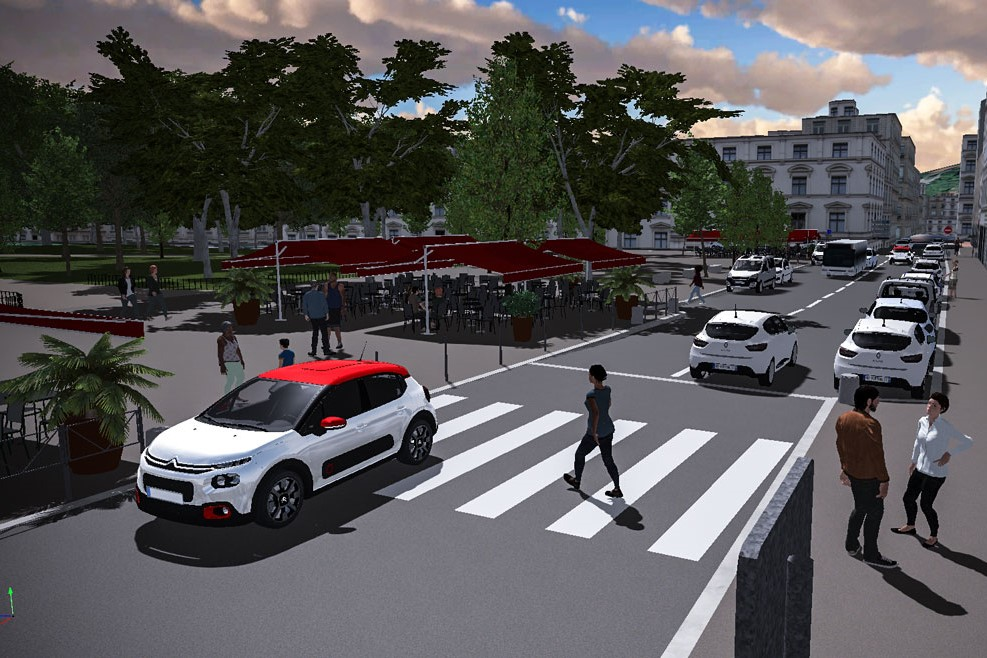
\includegraphics[width=0.5\textwidth]{Simulators/4DV-Sim.jpg}
    \caption{Source: \url{https://www.4d-virtualiz.com/en/automotive-simulator}}
\end{figure}

%%%%%%%% AirSIM %%%%%%%%%%
\subsection{AirSim} \label{AirSimDoc}
\textbf{Description:} AirSim\footnote{Website: \url{https://microsoft.github.io/AirSim}} is a simulator for cars and drones. It is open-source and works as a plugin for Unreal Engine, which means the simulator can be used with any environment which has been modeled inside the game engine. According to their website \cite{AirSim_Website}, the goal of the simulator is to create a platform for AI research to experiment with deep learning, computer vision, and reinforcement learning algorithms for autonomous systems. 

\textbf{Open Source:} Yes

\textbf{Operating System:} Any operating system

\textbf{Game Engine:} Primarily Unreal Engine, but it also offers a prototype version in Unity

\textbf{Pros:} Offers a large range of existing APIs. The simulator also has an active community on both discord and Github. It also gives the option to add drones. It is also designed to train machine learning models on it.

\textbf{Cons:} The simulator is not as realistic as other simulators. The vehicle physics is not as good as some of the other simulators, for example the handling and collisions. Also, currently, there are no pedestrians in the game. 

\textbf{Conclusion:} AirSim is worth looking closer into. As it is built using a game engine it should not be too hard to add the missing features, like for example adding and controlling pedestrians. In addition, as it is a plugin for Unreal Engine means that we can use other tools to import for example maps. Also, realistic vehicle physics was determined not to be an important factor for this project. 

\begin{figure}[H]
    \centering
    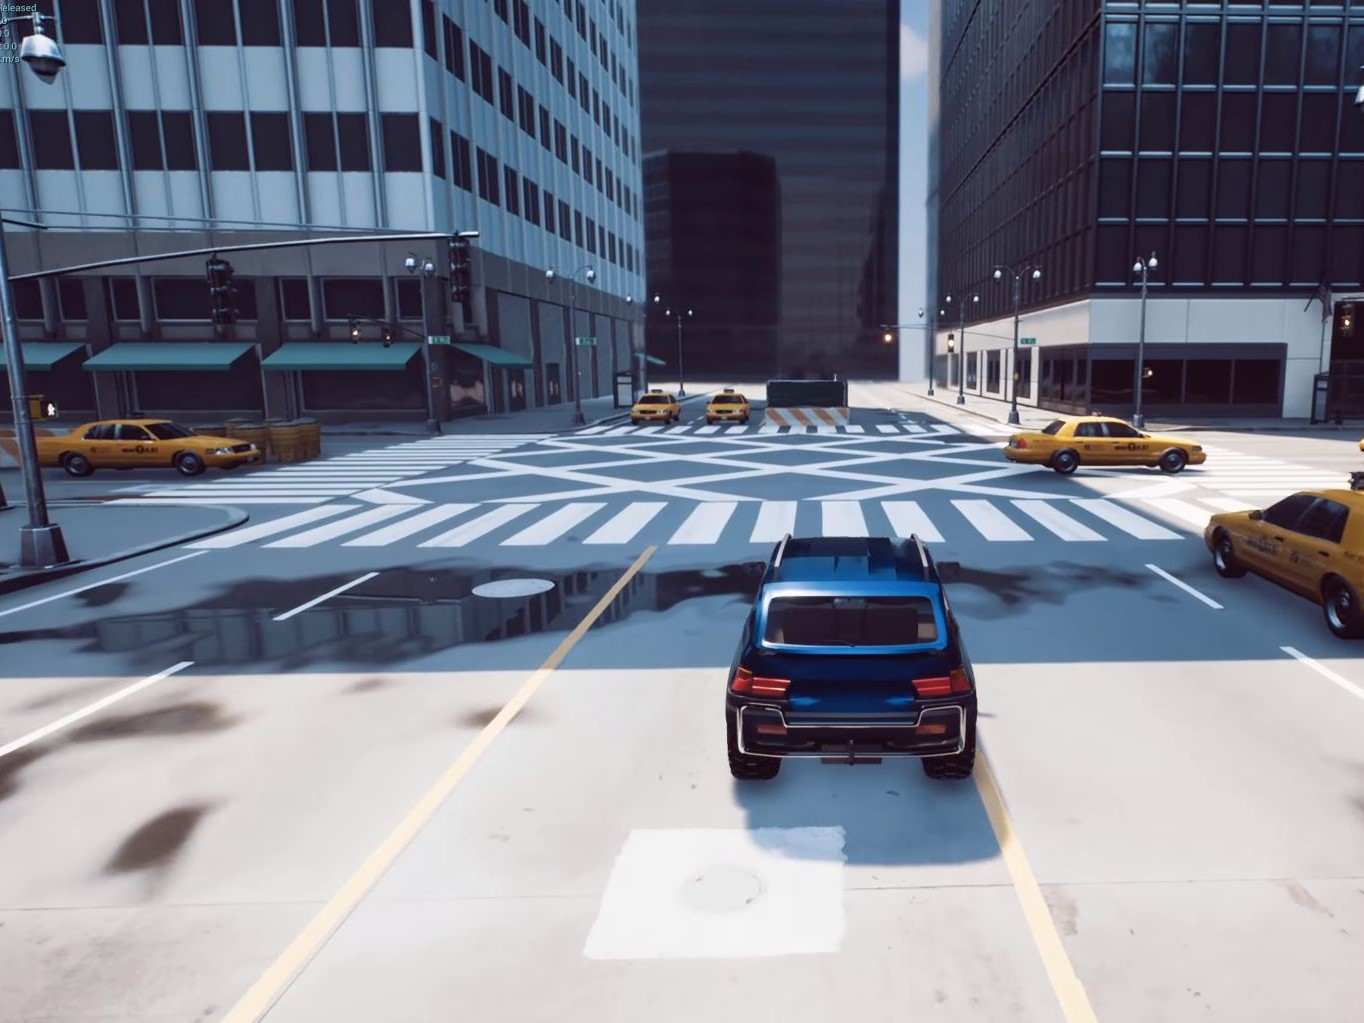
\includegraphics[width=0.5\textwidth]{Simulators/AirSim.JPG}
    \caption{Source: \url{https://microsoft.github.io/AirSim}}
\end{figure}

%%%%%%%% Apollo %%%%%%%%%%
\subsection{Apollo} \label{Apollo}
\textbf{Description:} Apollo\footnote{\url{https://github.com/ApolloAuto/apollo}} is a simulator that is designed to emulate the hardware in autonomous vehicles so that it can be trained for machine learning models. According to their website \cite{Apollo_Website}, Apollo is a flexible architecture that accelerates the development and testing of autonomous vehicles.

\textbf{Open Source:} Yes

\textbf{Operating System:} Any system that can run Docker

\textbf{Game Engine:} Unity

\textbf{Pros:} Accurately models the vehicle physics to help improve the machine learning model's accuracy. The simulator is also actively being worked on by a large community.  

\textbf{Cons:} It looks like quite a complex simulator, and it does therefore not seem like it will be easy to modify. The product is really specific towards training autonomous vehicles. 

\textbf{Conclusion:} Due to the complexity of this simulator, it does not look like something that we could build upon for this project. 

\begin{figure}[H]
    \centering
    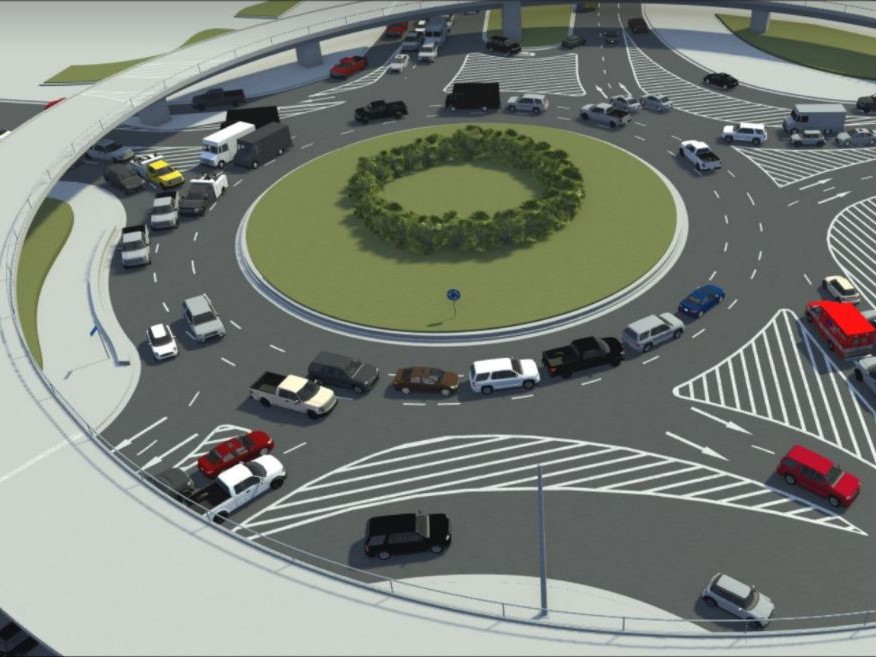
\includegraphics[width=0.5\textwidth]{Simulators/Apollo.JPG}
    \caption{Source: Slide deck from Apollo Game Engine Based Simulation Talk at GDC 2019 - \url{https://bit.ly/2VSzwlF}}
\end{figure}

%%%%%%%% Autoware %%%%%%%%%%
\subsection{Autoware} \label{Autoware}
\textbf{Description:} Autoware\footnote{\url{https://gitlab.com/autowarefoundation/autoware.auto/AutowareAuto}} is an open-source software for autonomous vehicles. It comes with a large variety of APIs  \cite{Autoware_doc_Website}. Autoware is however not a simulator, but can be used on a simulated vehicle to make it autonomous.

\textbf{Open Source:} Yes

\textbf{Operating System:} Robot Operating System (ROS)

\textbf{Game Engine:} Na

\textbf{Pros:} As it runs on ROS it can easily be adapted to work on a real autonomous vehicle.

\textbf{Cons:} Currently it only works with a specific car model and sensor set up. The software also seems quite complex, and combining it with a simulator will probably be quite challenging.

\textbf{Conclusion:} As this is not a simulator this is not something that we can use for this project. We will see with the LGSVL simulator (\ref{LGSVL_Simulator}), this software can be used alongside a simulator to model the autonomous system. 


%%%%%%%% Carla %%%%%%%%%%
\subsection{Carla} \label{Carla}
\textbf{Description:} Carla\footnote{\url{https://carla.org/}} is an open-source simulator for developing autonomous vehicles. It contains a variety of APIs and is actively being developed. Carla is also designed for training machine learning models \cite{CarlaPaper}. 

\textbf{Open Source:} Yes

\textbf{Operating System:} Primarily Linux, but also Windows

\textbf{Game Engine:} Unreal Engine

\textbf{Pros:} Has a lot of features already implemented, such as sensors, vehicle API, and the ability to add new objects. The simulator also has the ability to add pedestrians and plot their movement. Active community. Well documented and lots of information online. 

\textbf{Cons:} Difficult to add new and custom maps. Vehicle handling is not as realistic as some of the other simulators.

\textbf{Conclusion:} Carla is worth looking into further as it has most of the features that we are looking for.


\begin{figure}[H]
    \centering
    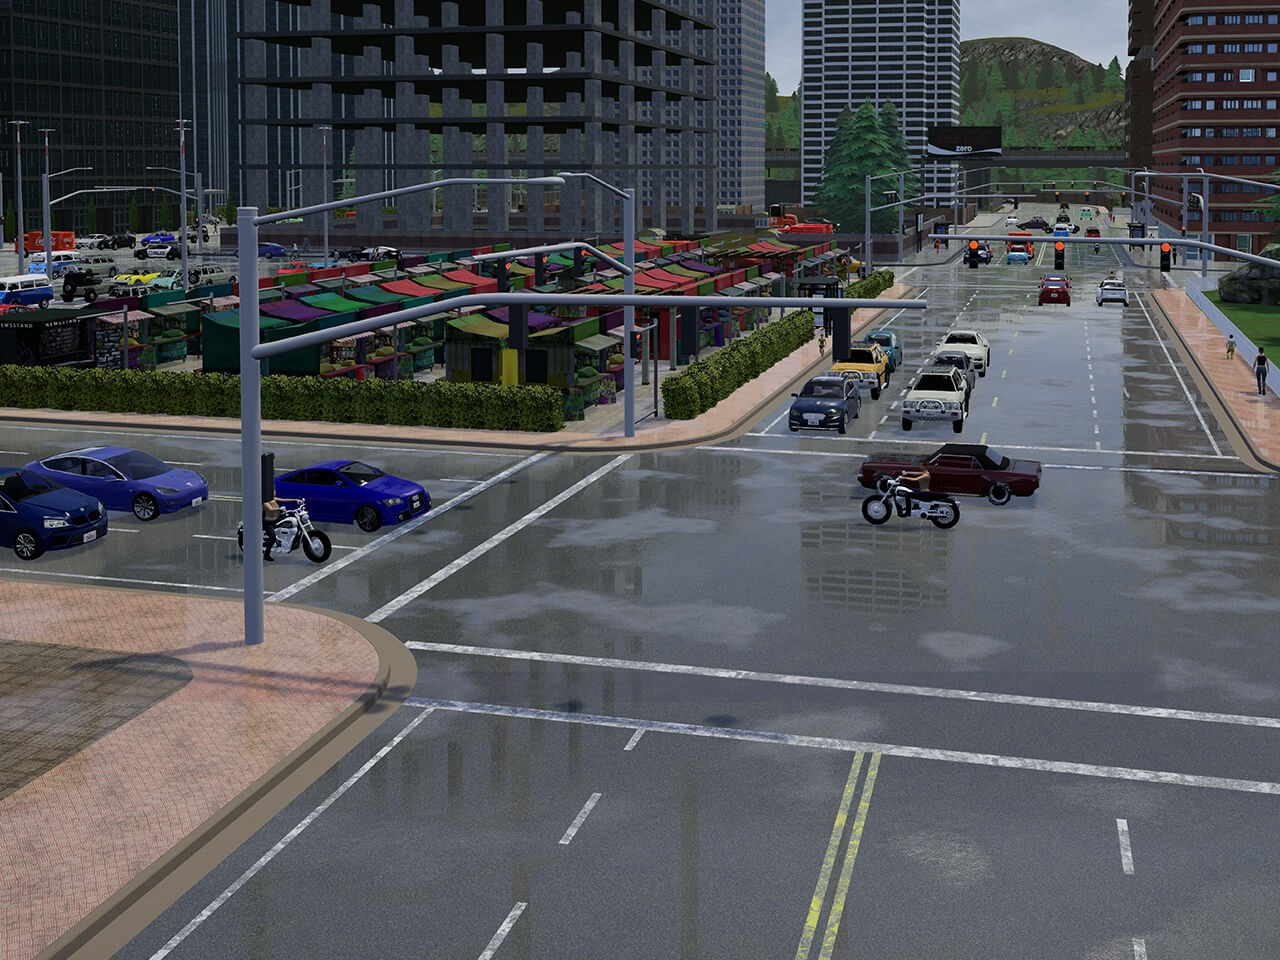
\includegraphics[width=0.5\textwidth]{Simulators/Carla.JPG}
    \caption{Source: \url{https://www.unrealengine.com/en-US/spotlights/carla-democratizes-autonomous-vehicle-r-d-with-free-open-source-simulator}}
\end{figure}


%%%%%%%% CrowdSim3D %%%%%%%%%%
\subsection{CrowdSim3D}
\textbf{Description:} CrowdSim3D\footnote{\url{https://crowdsim3d.com}} is primarily a simulator for modeling large crowds, but can also be used for vehicle traffic. 

\textbf{Open Source:} No (£180)

\textbf{Operating System:} Any operating system

\textbf{Game Engine:} Not specified

\textbf{Pros:} Has the ability to control several pedestrians and vehicles in a shared space.

\textbf{Cons:} Does not look to be designed for machine learning models. Difficult to add new models. Also, as it is not open source it will not be possible to customise the product. 

\textbf{Conclusion:} CrowdSim3D is not worth considering as we cannot adapt the product as it is not open source. 

\begin{figure}[H]
    \centering
    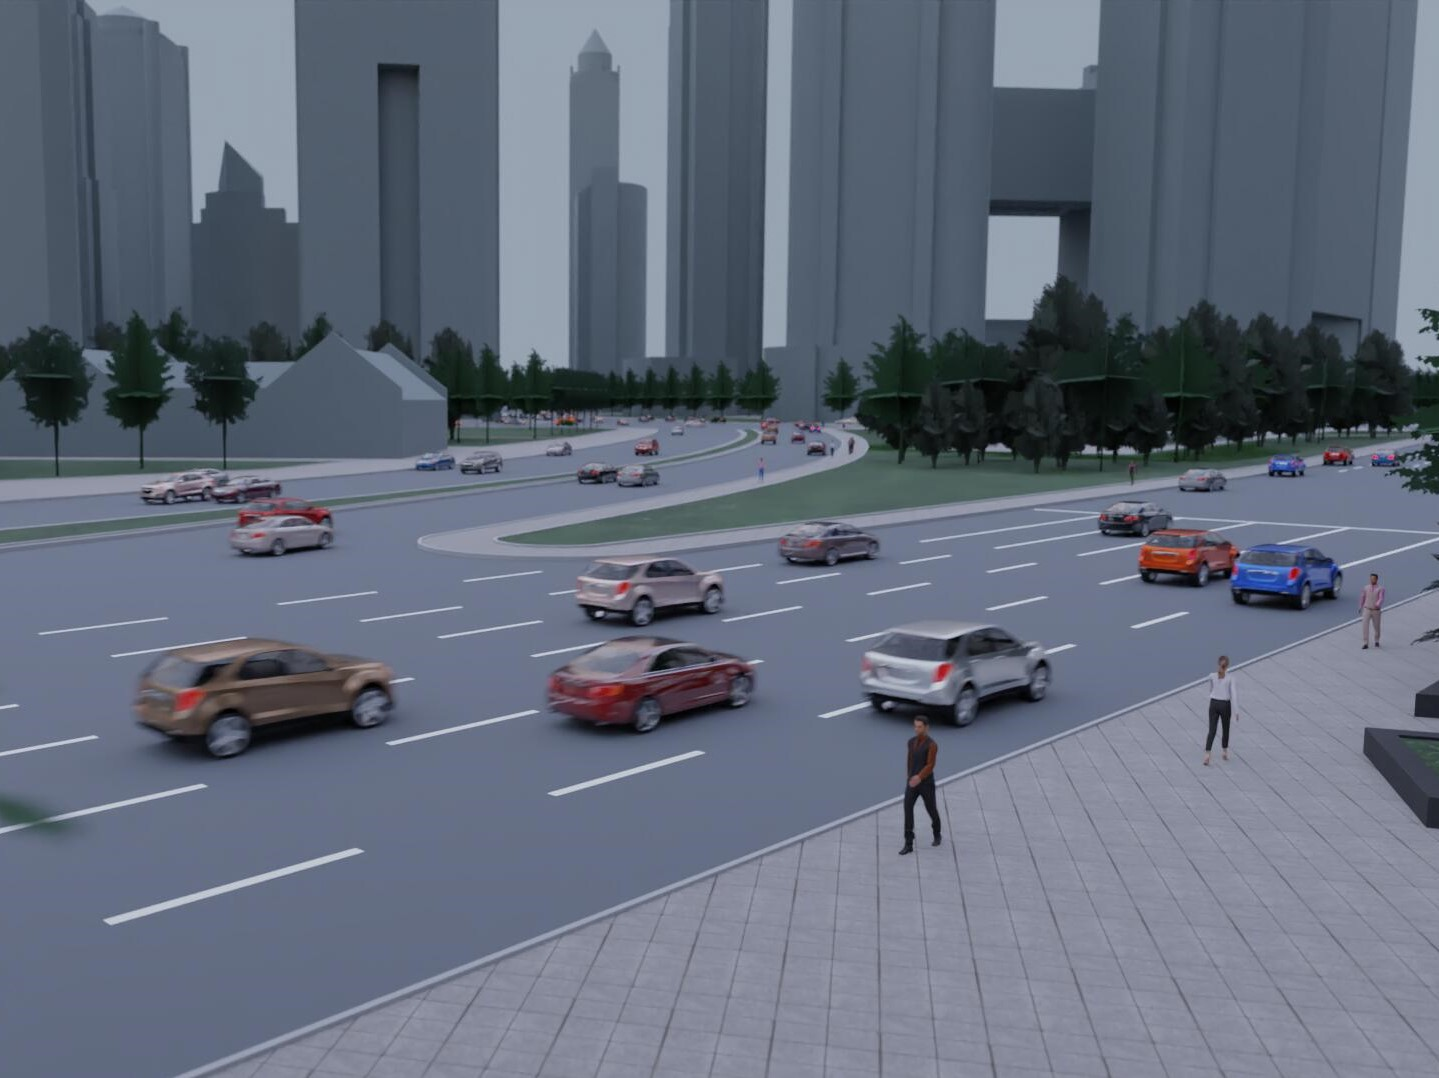
\includegraphics[width=0.5\textwidth]{Simulators/CrowdSim.JPG}
    \caption{Source: \url{https://crowdsim3d.com}}
\end{figure}


%%%%%%%% Deep Drive %%%%%%%%%%
\subsection{Deep Drive}
\textbf{Description:} Deep Drive\footnote{\url{https://deepdrive.voyage.auto/}} is an open-source simulator aimed to train neural networks for self-driving cars \cite{DeepDrive_Website}. They also provide you with a large data set to train your autonomous vehicle on. 

\textbf{Open Source:} yes

\textbf{Operating System:} Any operating system

\textbf{Game Engine:} Unreal Engine

\textbf{Pros:} Is able to handle a variety of different sensors and vehicle setups. It also has an active community and a leader board where you can compare your trained neural network against other developers. 

\textbf{Cons:} Currently there are three maps available, but it is not easy to add your own maps. Also, it is not designed to be customised. Currently, there are no pedestrians and no APIs.

\textbf{Conclusion:} Deep Drive is not a simulator that is worth looking at as it is not designed to be customised. It also lacks most of the features we are looking for. 

\begin{figure}[H]
    \centering
    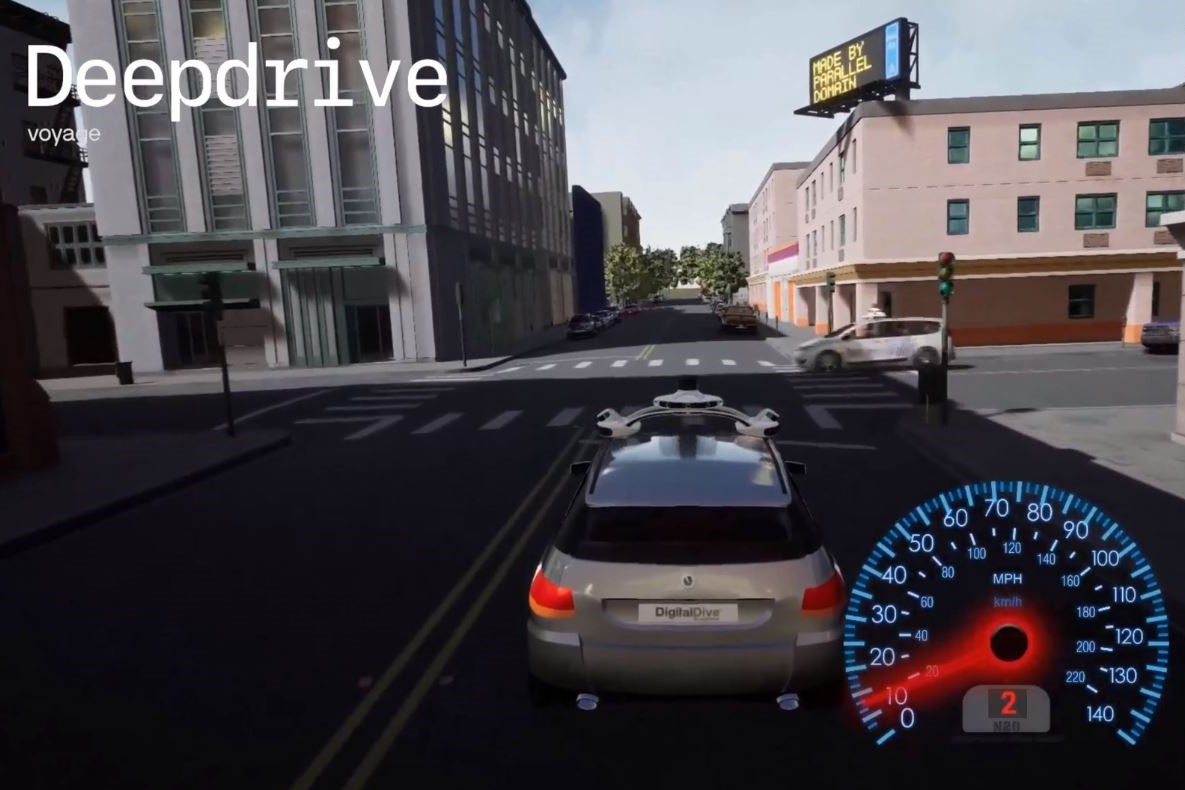
\includegraphics[width=0.5\textwidth]{Simulators/DeepDrive.JPG}
    \caption{Source: \url{https://deepdrive.voyage.auto}}
\end{figure}

%%%%%%%% Donkey Car Simulator %%%%%%%%%%
\subsection{Donkey Car Simulator}
\textbf{Description:} Donkey Car Simulator\footnote{\url{https://docs.donkeycar.com/guide/simulator}} is a simulator for the Donkey Car. The car itself costs roughly £200 and can be ordered online, or you can download the schematics for free. The simulator can be used to train a neural network in Python which can then run on your car. 

\textbf{Open Source:} Yes

\textbf{Operating System:} Any operating system

\textbf{Game Engine:} Unity

\textbf{Pros:} Easy to use

\textbf{Cons:} Not what we are looking for as it is only used to train a real toy car.

\textbf{Conclusion:} Donkey Car is an interesting project to read about as it is a fun kit that introduces people to autonomous cars. However, it is not what we are looking for for this project as the simulator is not customisable and there is only one vehicle. 


\begin{figure}[H]
    \centering
    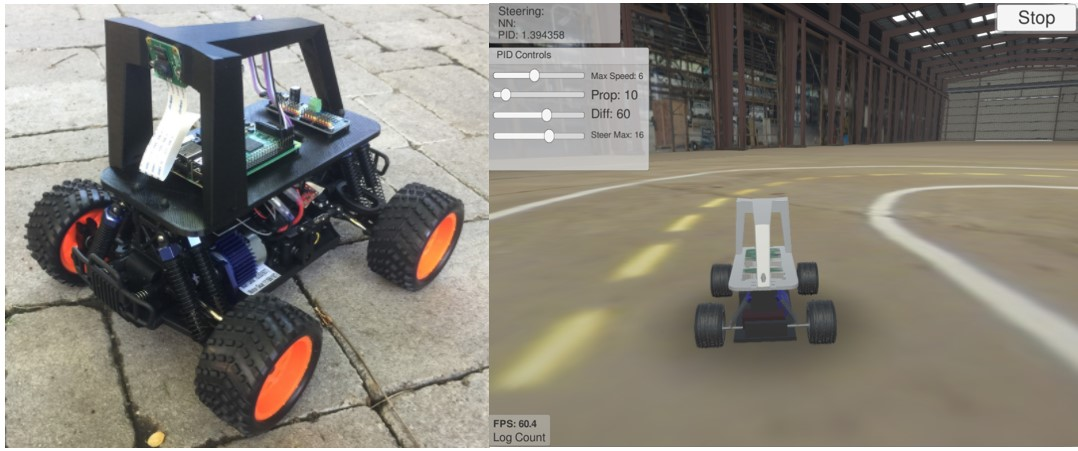
\includegraphics[width=0.5\textwidth]{Simulators/DonkeySim.jpg}
    \caption{Source: \url{https://docs.donkeycar.com}}
\end{figure}

%%%%%%%% Gazebo %%%%%%%%%%
\subsection{Gazebo}\label{gazebo}
\textbf{Description:} Gazebo\footnote{\url{http://gazebosim.org}} is a robotics simulator designed to design robots, test algorithms and train AI systems \cite{Gazebo_Website}. Gazebo offers the ability to simulate several robots at once in both indoor and outdoor environments.

\textbf{Open Source:} Yes

\textbf{Operating System:} Any operating system

\textbf{Game Engine:} ODE, but also Bullet, Simbody and DART which are additional physics engines. 

\textbf{Pros:} Very versatile, can be used for much more than traffic simulations. 

\textbf{Cons:} Due to the large number of different physics engines it might be complicated to fix something if a feature breaks. The documentations is not as clear as some other simulators. 

\textbf{Conclusion:} Gazebo is worth looking at as it is widely used for robotics simulations. All the sensing APIs are already implemented.


\begin{figure}[H]
    \centering
    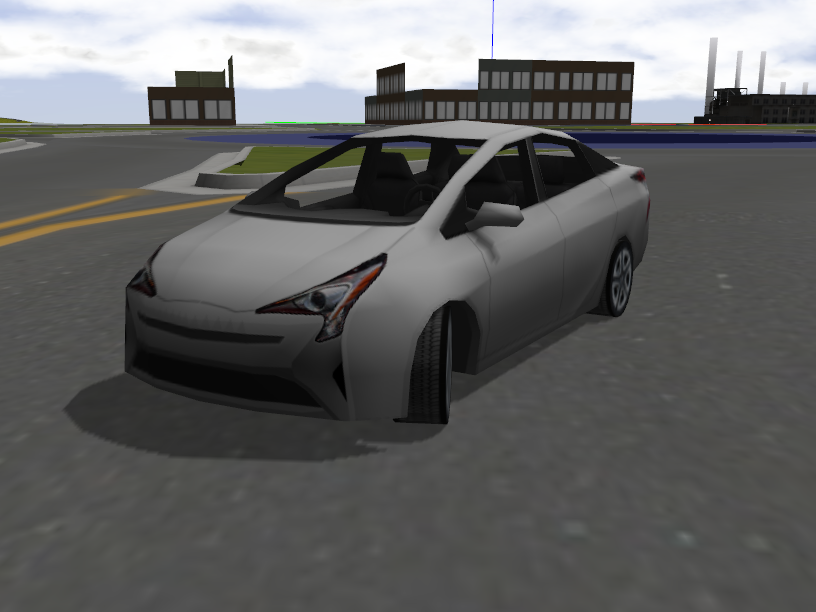
\includegraphics[width=0.5\textwidth]{Simulators/gazebo.png}
    \caption{Source: \url{http://gazebosim.org/blog/vehicle\%20simulation}}
\end{figure}


%%%%%%%% LPZRobots %%%%%%%%%%
\subsection{LPZRobots}
\textbf{Description:} LPZRobots\footnote{\url{https://github.com/georgmartius/lpzrobots}} is a robotics simulator created by the Robotics Group for Self-Organisation of Control at the University of Leipzig in Germany \cite{LPZRobots_Website, LPZRobots_book}. The simulator aims to have an open environment to simulate the robot's physics. 

\textbf{Open Source:} Yes

\textbf{Operating System:} Primarily Linux, but now also supports Windows

\textbf{Game Engine:} ODE

\textbf{Pros:} Free to add any kind of robot.

\textbf{Cons:} The code has not been updated since 2018 and the last release was in 2016. Unlike other simulators, this one does not seem to have an active community. 

\textbf{Conclusion:} As the development of the LPZRobots simulator has been inactive for several years, makes it not worth considering. The simulator also lacks most of the features we are looking for. 

\begin{figure}[H]
    \centering
    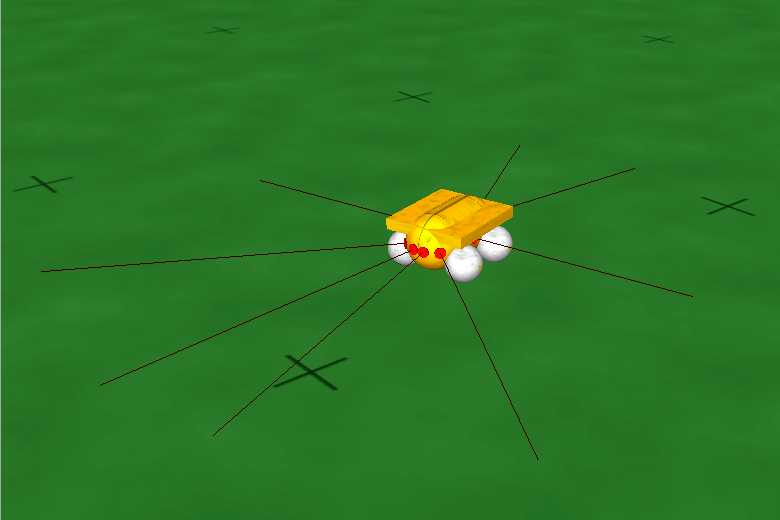
\includegraphics[width=0.5\textwidth]{Simulators/LPZRobots.png}
    \caption{Source: \url{https://itp.uni-frankfurt.de/~gros/StudentProjects/Robots\_2016\_ObstacleAvoidance}}
\end{figure}


%%%%%%%% LGSVL Simulator %%%%%%%%%%
\subsection{LGSVL Simulator} \label{LGSVL_Simulator}
\textbf{Description:} LGSVL\footnote{\url{https://github.com/lgsvl/simulator}} is a simulator created by the Advanced Platform Lab at the LG Electronics America R\&D Center \cite{LGSVL_Web}. The simulator combines the vehicle from Autoware (Section~\ref{Autoware}) with Apollo (Section~\ref{Apollo}) which emulates the hardware. The LGSVL has lots of available APIs such as cameras, LiDAR, RADAR, and GPS. Some environmental parameters can also be changed such as the map, weather, and pedestrians.
% Uses Apollo and Autoware

\textbf{Open Source:} Yes

\textbf{Operating System:} Windows 10

\textbf{Game Engine:} A variety due to its complexness, but both Unreal Engine and Unity.

\textbf{Pros:} Has most of the features we are looking for.

\textbf{Cons:} Relies on a lot of different components. The codebase is therefore large and complex and it looks difficult to add our own features such as our own entity.

\textbf{Conclusion:} The LGSVL Simulator would probably not work for us as the code-base seems too large and complex.

\begin{figure}[H]
    \centering
    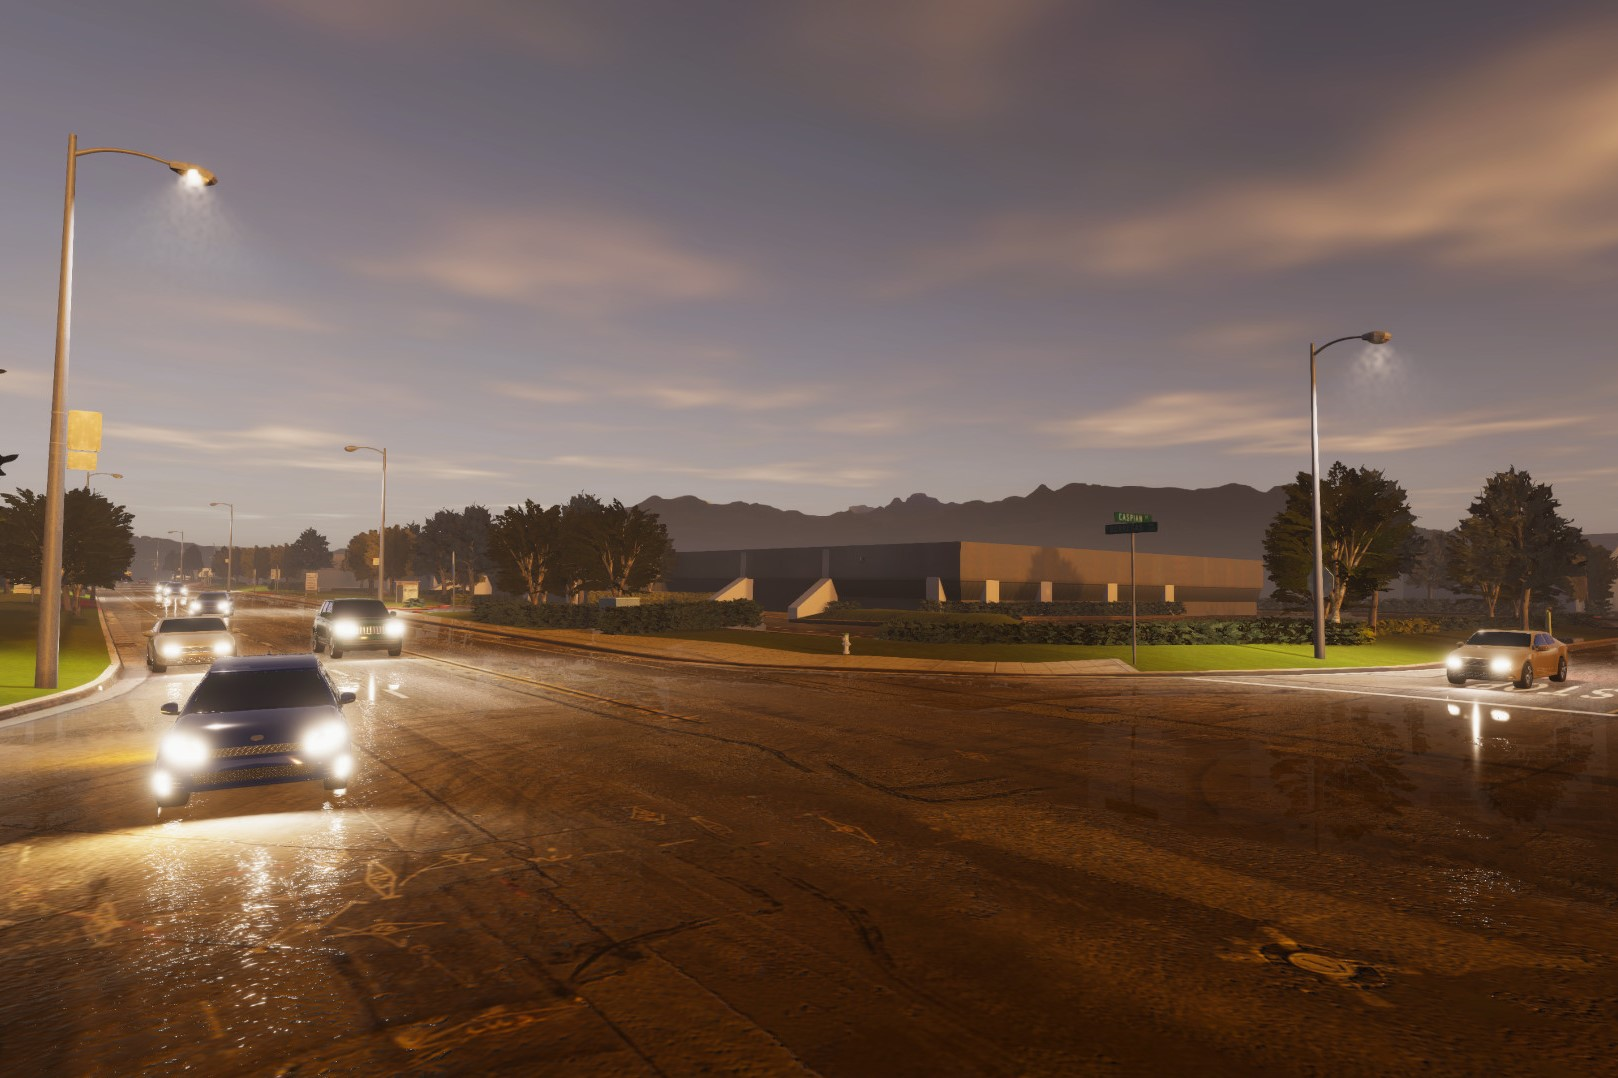
\includegraphics[width=0.5\textwidth]{Simulators/LGSVL.jpg}
    \caption{Source: \url{https://www.lgsvlsimulator.com/about}}
\end{figure}
%https://github.com/lgsvl/simulator

%%%%%%%% Marilou %%%%%%%%%%
\subsection{Marilou}
\textbf{Description:} Marilou\footnote{\url{http://www.anykode.com/index.php}} is a simulator created by ANYKODE \cite{Marilou_Web}. Marilou is an open map simulator where the user can add objects and hindrances for the robot to navigate around. The simulator is designed to simulate simultaneous localisation and mapping (SLAM) and other localisation techniques. 

\textbf{Open Source:} No (£350)

\textbf{Operating System:} Windows and Linux

\textbf{Game Engine:} Unknown

\textbf{Pros:} Accurately simulates sensors and robot behavior. Easy to add new objects and other controllable entities. 

\textbf{Cons:} As the simulator is not open source, we cannot modify its behavior. Latest release 2018.

\textbf{Conclusion:} Marilou is not a simulator that we can use for this project as it is not open source. In addition, it is not designed with APIs in mind and controlling multiple objects at once looks impossible in the current program. 

\begin{figure}[H]
    \centering
    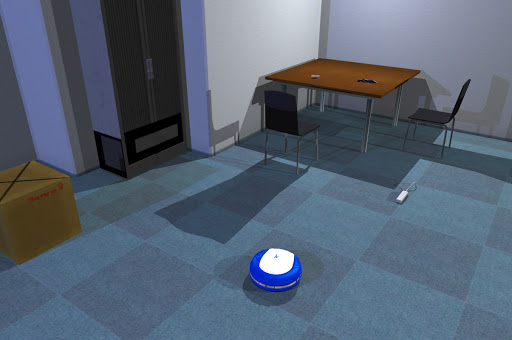
\includegraphics[width=0.5\textwidth]{Simulators/Marilou.jpg}
    \caption{Source: \url{http://www.anykode.com/downloads.php}}
\end{figure}


%%%%%%%% rFpro %%%%%%%%%%
\subsection{rFpro}
\textbf{Description:} rFpro\footnote{\url{https://www.rfpro.com}} is a driving simulation software which focuses on road-vehicle simulation \cite{rFpro_Web}. rFpro allows for a variety of use cases, from training machine learning models for autonomous driving \cite{rFpro_ML}, to motor racing.

\textbf{Open Source:} No

\textbf{Operating System:} Windows

\textbf{Game Engine:} ISIMotor - A game engine created by Image Space Inc \cite{ISIMotor}. The game engine is used for F1 and other racing games.

\textbf{Pros:} A professionally made simulator that has most of the features we are looking for. Very good graphics and accurate vehicle behavior. 

\textbf{Cons:} rFpro does not give us access to any of the source code. The price is only available upon request, but it is most likely too expensive for this project. 

\textbf{Conclusion:} Even though rFpro contains just about all of the features we are looking for, and is probably the best-looking simulator, it will not work for this project as it is not open source. 

\begin{figure}[H]
    \centering
    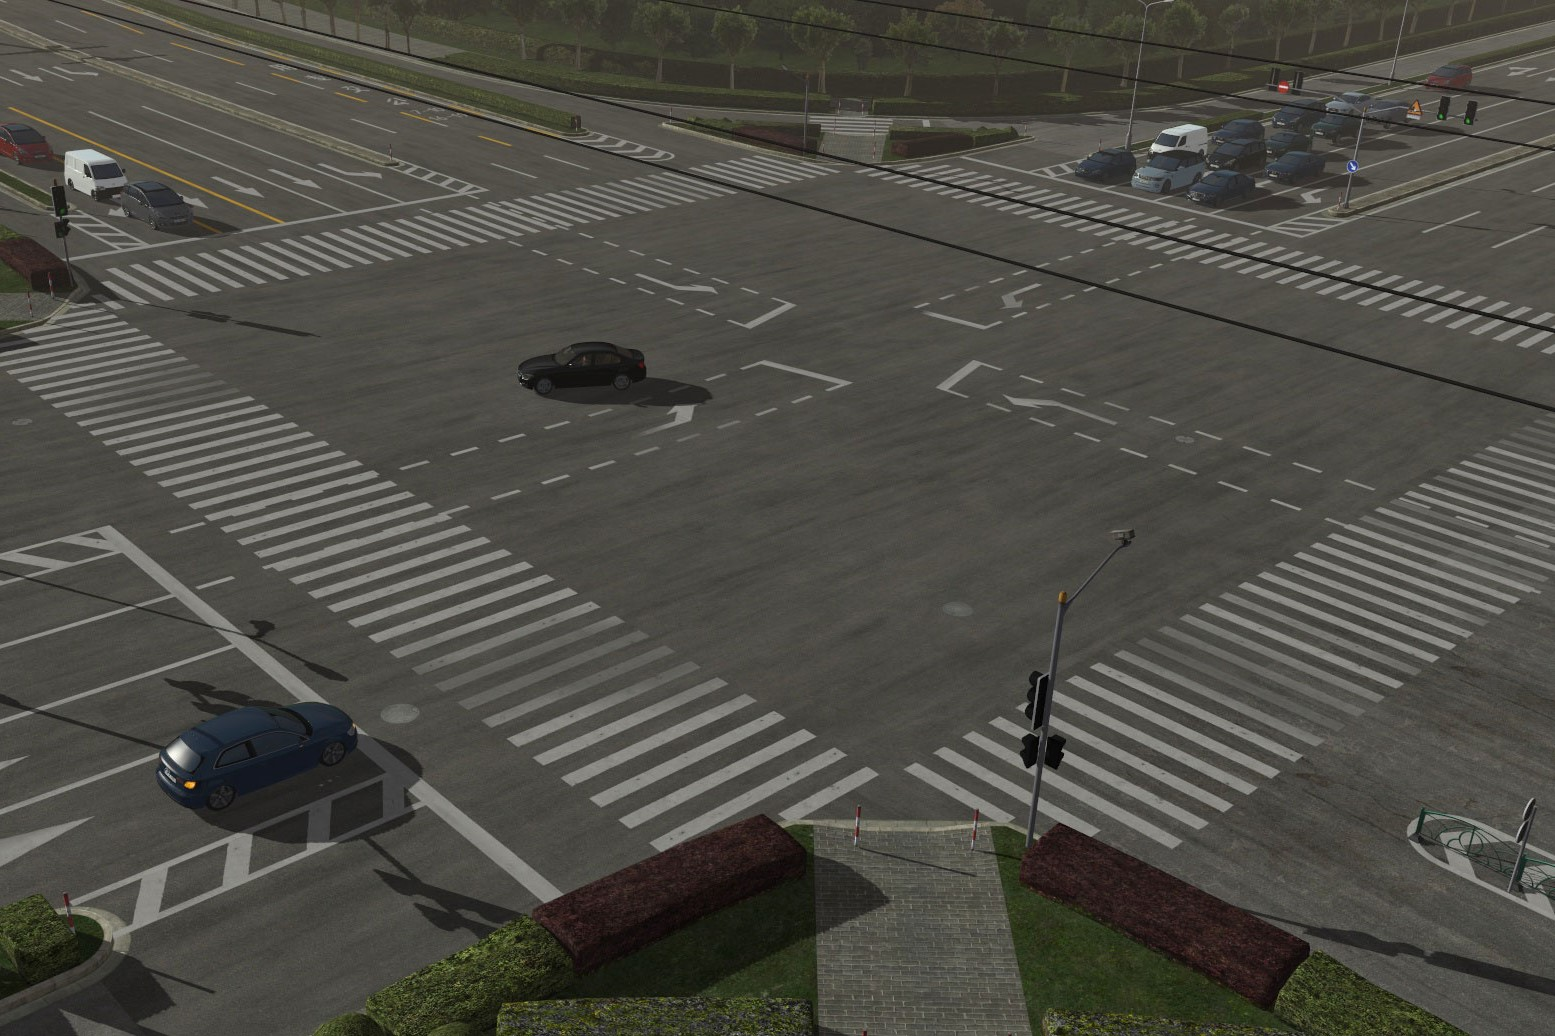
\includegraphics[width=0.5\textwidth]{Simulators/rFpro.jpg}
    \caption{Source: \url{http:https://www.rfpro.com/driving-simulation}}
\end{figure}

%%%%%%%% Rigs of Rods %%%%%%%%%%
\subsection{Rigs of Rods}
\textbf{Description:} Rigs of Rods\footnote{\url{https://www.rigsofrods.org}} (RoR) is an open-source physics simulator primarily designed to simulate vehicle physics. The simulator uses soft-body physics which means that if the vehicle collides, its structure will be deformed. This will result in a more accurate simulation.

\textbf{Open Source:} Yes

\textbf{Operating System:} Windows and Linux

\textbf{Game Engine:} Non, creates its own soft-body physics engine.

\textbf{Pros:} There is an active community creating modifications for the simulator. Also, the only simulator on the list which uses soft-body physics. 

\textbf{Cons:} There are no APIs currently available. 

\textbf{Conclusion:} As for this project, we are not looking for realistic features, but rather certain APIs. This simulator will require too much work to add the missing features. It is therefore not a simulator that is worth considering. 

\begin{figure}[H]
    \centering
    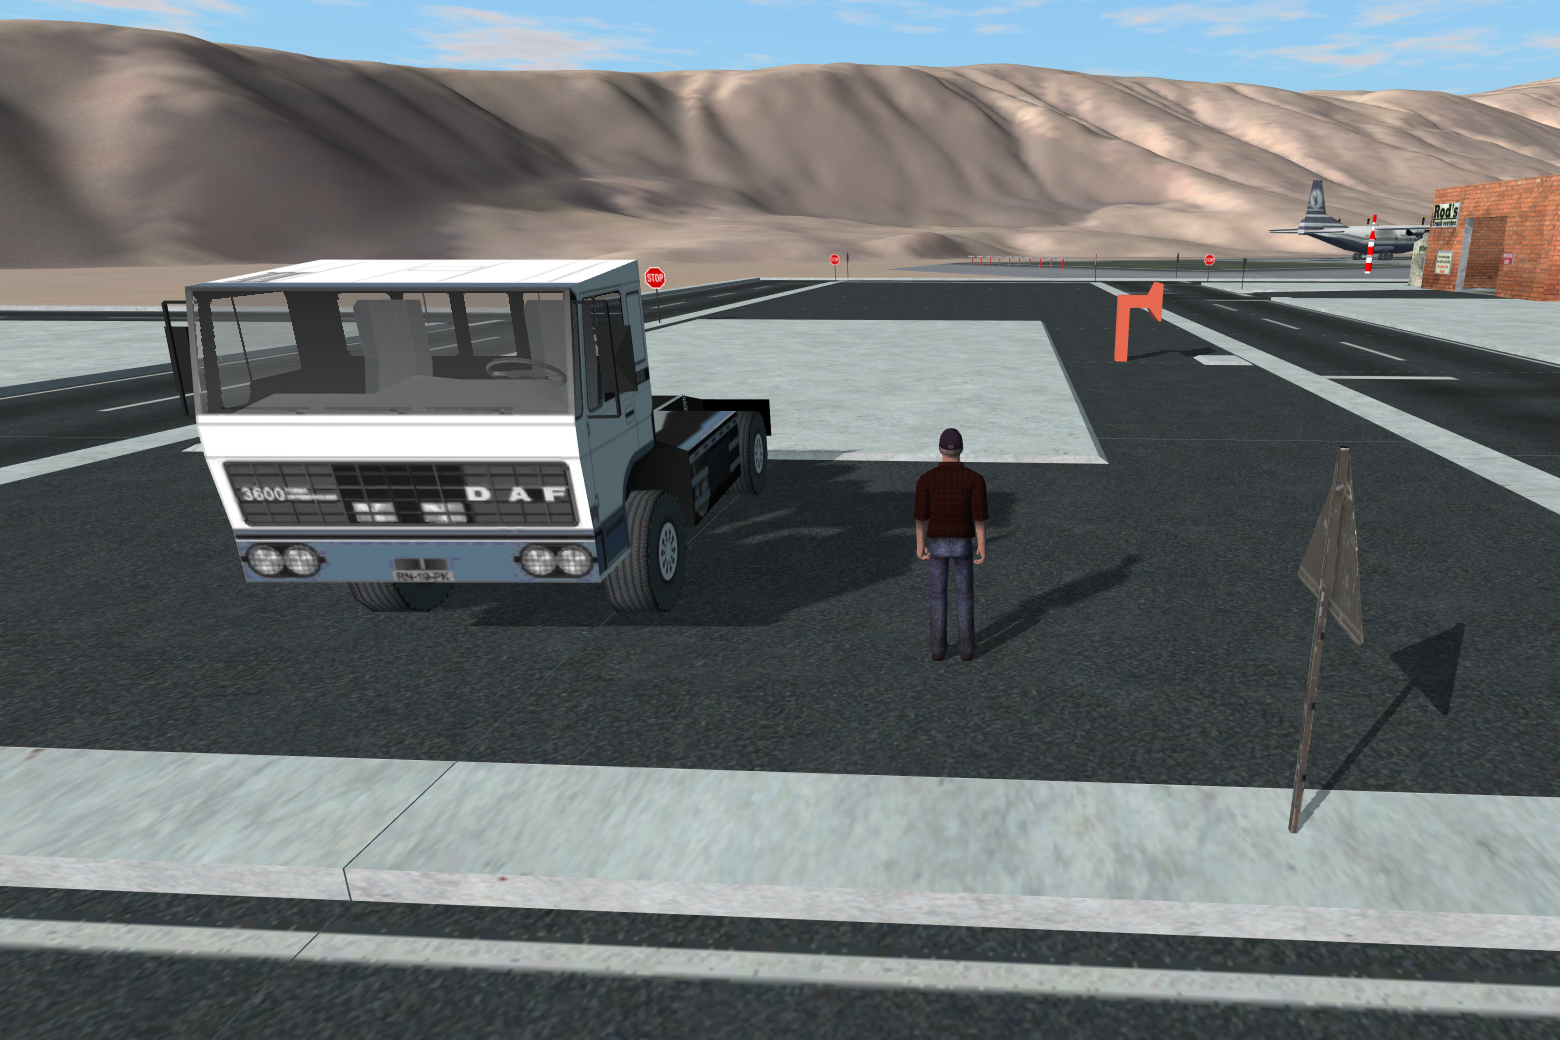
\includegraphics[width=0.5\textwidth]{Simulators/RoR.png}
    \caption{Source: \url{https://docs.rigsofrods.org/gameplay/beginners-guide}}
\end{figure}


%%%%%%%% TORCS - The Open Racing Car Simulator %%%%%%%%%%
\subsection{TORCS - The Open Racing Car Simulator}
\textbf{Description:} TORCS\footnote{\url{https://sourceforge.net/projects/torcs}} is an open-source racing car simulator. It can be used as an ordinary racing game or as an AI racing research platform. The creators of TORCS used to host competitions on its website among players for who could create the best artificially intelligent racing car \cite{TORCS_Racing}. 

\textbf{Open Source:} Yes

\textbf{Operating System:} Linux and Windows

\textbf{Game Engine:} Non, implemented from scratch.

\textbf{Pros:} Easy to add and create new content. 

\textbf{Cons:} Latest release 2016 but mainly developed in 2008. Also, has no available APIs and no pedestrians.

\textbf{Conclusion:} This simulator is lacking most of the features we are looking for. It is also quite outdated. TORCS is therefore not worth considering. 

\begin{figure}[H]
    \centering
    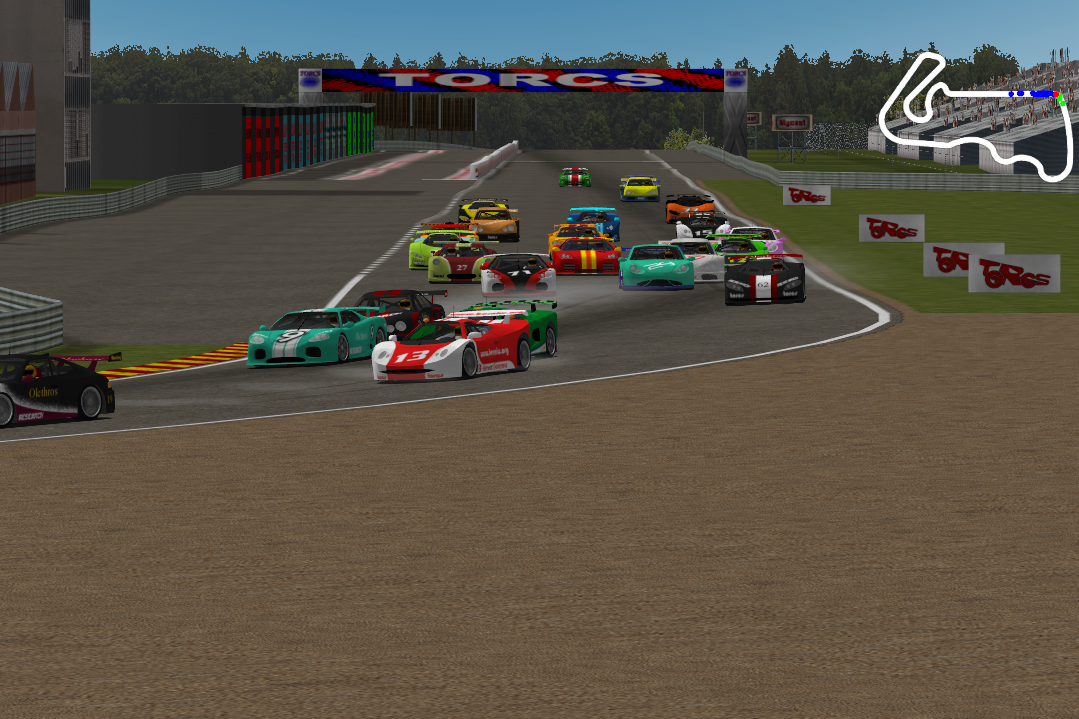
\includegraphics[width=0.5\textwidth]{Simulators/TORCS.png}
    \caption{Source: \url{https://sourceforge.net/projects/torcs}}
\end{figure}

%%%%%%%% Webots %%%%%%%%%%
\subsection{Webots}
\textbf{Description:} Webots\footnote{\url{https://www.cyberbotics.com}} is an open-source robotics simulator developed by Cyberbotics \cite{Webots_Github}. Webots provides a complete developing environment to model, program and simulate the robots \cite{Webots_home}. 

\textbf{Open Source:} Yes

\textbf{Operating System:} Any operating system

\textbf{Game Engine:} ODE

\textbf{Pros:} A lot of documentation on how to add new features. Seems to be able to generate new maps easily. Available chat page.

\textbf{Cons:} There does not seem to be many APIs to control multiple entities. All the APIs are mainly used for sensing. 

\textbf{Conclusion:} Webots has most of the features that we are looking for, however seems to lack the ability to easily control multiple entities at once. The simulator also seems less advanced than Gazebo (Section~\ref{gazebo}), so as an open area robotics simulator, we will rather look at that one first. We will therefore not be considering Webots.

\begin{figure}[H]
    \centering
    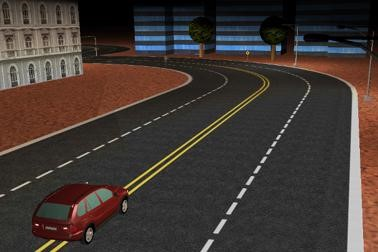
\includegraphics[width=0.5\textwidth]{Simulators/Webots.jpg}
    \caption{Source: \url{https://www.cyberbotics.com/doc/automobile/city-night}}
\end{figure}

\subsection{Conclusion}
After looking at the different simulators we decided to look further into AirSim (Section~\ref{AirSimDoc}), Carla (Section~\ref{Carla}) and Gazebo (Section~\ref{gazebo}). These are the simulators that will hopefully be the easiest to adapt and modify to suit our needs. In the next section, Analysis of Competing Product (Section~\ref{AoCP}), we will look at which of these three simulators to go for. 
%https://www.hisour.com/robotics-simulator-42971/
